\raggedbottom
\chapter{Análisis de requisitos}
En esta sección se tratará de analizar todos los requisitos que necesitará cumplir rigurosamente nuestra aplicación software.
\section{Análisis de implicados}
Es importante identificar a los interesados en el sistema. En este sistema habrá 3 implicados: enviadores, transportistas y receptores, se procede a describir de forma breve la interacción de cada uno de estos implicados:


\begin{table}[H]
    \centering
    \small
    \begin{tabularx}{\textwidth}{|p{2.5cm}|X|p{2.5cm}|X|}
        \hline
        \textbf{Nombre} & \textbf{Descripción} & \textbf{Tipo} & \textbf{Responsabilidad} \\ \hline
        Enviador & Representa al usuario responsable de organizar y gestionar el envío de remesas. & Usuario producto & Programar los envíos, gestionar las remesas en el sistema y dar de alta a los transportistas y medios de transporte asociados. \\ \hline
        Transportista & Representa al usuario encargado de transportar las remesas asignadas. & Usuario producto & Consultar sus horarios y rutas en el sistema, así como programar y seguir las planificaciones de entrega asignadas. \\ \hline
        Destinatario & Representa al usuario final que recibirá las remesas enviadas. & Usuario producto y sistema & Consultar en tiempo real el estado de su remesa y monitorizar su ubicación y progreso durante todo el proceso de entrega. \\ \hline
        Usuario & Representa a cualquier usuario del sistema (enviador, transportista o destinatario). & Usuario general & Acceder a funcionalidades comunes como la autenticación, la gestión del perfil o la recepción de notificaciones. \\ \hline
        Sistema (Aplicación) & Núcleo de la aplicación que gestiona los flujos internos y coordina la interacción con usuarios y servicios externos. & Sistema & Ejecutar operaciones lógicas internas y comunicarse con el subsistema blockchain para registrar eventos importantes. \\ \hline
    \end{tabularx}
    \caption{Actores del sistema y sus responsabilidades}
    \normalsize
\end{table}



Aclarar que al utilizar la tecnología blockchain todos los implicados podrán consultar el estado de la remesa en el momento que lo deseen de manera segura y transparente, sin embargo esta funcionalidad a pesar de ser muy útil para todos los implicados es la que le proporcionará total confianza al destinatario.

\section{Requisitos Funcionales}
Estos requisitos según \href{https://clickup.com/es-ES/blog/138879/analisis-de-requisitos}{ClickUp} Son las funcionalidades que debe ofrecer el software desarrollado. Durante el proceso de análisis se han identificado un total de 22 requisitos funcionales, organizados en función de las áreas a las que hacen referencia. 
Cada requisito funcional identificado contará con una estimación en puntos de historia, los cuales servirán como referencia para valorar el esfuerzo necesario —en términos de tiempo ideal— para su implementación. Estos puntos están basados en la secuencia de Fibonacci. Es importante destacar que un requisito con el doble de puntuación que otro no implica necesariamente el doble de tiempo de desarrollo, sino que representa el doble de esfuerzo relativo.
Se seguirá una escala de puntuación común en metodologías ágiles como está:\\


% Definimos una nueva columna centrada con padding
\newcolumntype{C}[1]{>{\centering\arraybackslash}p{#1}}

\begin{table}[H]
    \centering
    \renewcommand{\arraystretch}{1.5} % Aumenta el alto de las filas
    \begin{tabular}{|C{4cm}|C{10cm}|}
        \hline
        \rowcolor[HTML]{3531FF} 
        {\color[HTML]{FFFFFF}\textbf{Puntos de historia}} & {\color[HTML]{FFFFFF}\textbf{Esfuerzo relativo necesario}} \\ \hline
        \cellcolor[HTML]{96FFFB} \textbf{1} & Tarea sencilla, bajo riesgo, sin complejidad \\ \hline
        \cellcolor[HTML]{9AFF99} \textbf{2} & Tarea simple pero con ligera complejidad \\ \hline
        \cellcolor[HTML]{FFFE65} \textbf{3} & Tarea intermedia, necesita más desarrollo y pruebas \\ \hline
        \cellcolor[HTML]{FE0000} \textbf{5} & Tarea compleja, con más incertidumbre técnica o lógica \\ \hline
    \end{tabular}
    \caption{Escala de puntos de historia y esfuerzo relativo}
\end{table}

A continuación, se presentará un resumen de todos los requisitos funcionales identificados, seguido de una descripción detallada de cada uno de ellos.

\begin{table}[H]
    \centering
    \scriptsize
    \renewcommand{\arraystretch}{1.2}
    \begin{tabular}{|c|c|p{4.8cm}|c|c|}
    \hline
    \textbf{Épica} & \textbf{Id} & \textbf{Descripción} & \textbf{Estimación} & \textbf{Prioridad} \\
    \hline
    \multirow{5}{*}{\rule{0pt}{13pt}\begin{tabular}[c]{@{}c@{}}Gestión\\ de\\ usuarios\\ \end{tabular}} 
    & RF-1 & \rule{0pt}{13pt}Los usuarios deben poder registrarse proporcionando su información personal. & 3 & Alta \\
    \cline{2-5}
    & RF-2 & \rule{0pt}{13pt}Los usuarios deben poder iniciar sesión utilizando sus credenciales. & 2 & Alta \\
    \cline{2-5}
    & RF-3 & \rule{0pt}{13pt}El sistema debe validar que la dirección de correo electrónico proporcionada sea válida. & 3 & Media \\
    \cline{2-5}
    & RF-4 & \rule{0pt}{13pt}Los usuarios deben poder modificar su información personal desde su perfil. & 2 & Alta \\
    \cline{2-5}
    & RF-5 & \rule{0pt}{13pt}Los usuarios deben poder cerrar sesión de forma segura en cualquier momento. & 1 & Alta \\
    \hline
    \multirow{4}{*}{\rule{0pt}{13pt}\begin{tabular}[c]{@{}c@{}}Gestión\\ de\\ remesas\end{tabular}} 
    & RF-6 & \rule{0pt}{13pt}El enviador debe poder crear nuevas remesas para su gestión y seguimiento. & 3 & Alta \\
    \cline{2-5}
    & RF-7 & \rule{0pt}{13pt}El enviador debe poder asignar manualmente transportistas responsables de cada remesa. & 3 & Alta \\
    \cline{2-5}
    & RF-8 & \rule{0pt}{13pt}El enviador debe poder consultar el historial completo de cada remesa. & 2 & Alta \\
    \cline{2-5}
    & RF-9 & \rule{0pt}{13pt}El enviador debe poder editar la información de una remesa previamente creada. & 3 & Alta \\
    \hline
    \multirow{2}{*}{\rule{0pt}{13pt}\begin{tabular}[c]{@{}c@{}}Gestión\\ de\\ seguimiento\\ y\\ localización\end{tabular}} 
    & RF-10 & \rule{0pt}{13pt}El usuario debe poder visualizar en tiempo real la ubicación y estado de su remesa. & 5 & Alta \\
    \cline{2-5}
    & RF-11 & \rule{0pt}{13pt}El usuario debe recibir notificaciones por correo electrónico sobre cambios en el estado de su remesa. & 3 & Alta \\
    \hline
    \multirow{4}{*}{\rule{0pt}{13pt}\begin{tabular}[c]{@{}c@{}}Gestión\\ de\\ transportistas\end{tabular}} 
    & RF-12 & \rule{0pt}{13pt}El transportista debe poder recibir asignaciones automáticas de remesas. & 3 & Alta \\
    \cline{2-5}
    & RF-13 & \rule{0pt}{13pt}El usuario debe poder actualizar el estado de la remesa durante su transporte. & 2 & Alta \\
    \cline{2-5}
    & RF-14 & \rule{0pt}{13pt}El transportista debe poder modificar su información personal. & 2 & Alta \\
    \cline{2-5}
    & RF-15 & \rule{0pt}{13pt}El transportista debe poder solicitar su baja del sistema cuando lo desee. & 1 & Alta \\
    \cline{2-5}
    & RF-16 & \rule{0pt}{13pt}El enviador debe poder dar de alta a un transportista en el sistema & 2 & Media \\
    \hline
    \multirow{2}{*}{\rule{0pt}{13pt}\begin{tabular}[c]{@{}c@{}}Gestión\\ de\\ estadísticas\\ y\\ reportes\end{tabular}}
    & RF-17 & \rule{0pt}{13pt}El enviador debe poder generar reportes sobre el estado de sus remesas (en tránsito, entregadas, retrasadas, etc.). & 3 & Alta \\
    \cline{2-5}
    & RF-18 & \rule{0pt}{13pt}El enviador debe poder visualizar estadísticas como el número de transportistas asignados, remesas generadas y otros datos relevantes. & 3 & Alta \\
    \hline
    \end{tabular}
    \caption{Tabla resumen requisitos funcionales}
\end{table}

\begin{table}[H]
    \centering
    \scriptsize
    \renewcommand{\arraystretch}{1.2}
    \begin{tabular}{|c|c|p{4.8cm}|c|c|}
    \hline
    \textbf{Épica} & \textbf{Id} & \textbf{Descripción} & \textbf{Estimación} & \textbf{Prioridad} \\
    \hline
    \multirow{4}{*}{\rule{0pt}{13pt}\begin{tabular}[c]{@{}c@{}}Gestión\\ de la\\ blockchain\end{tabular}} 
    & RF-19 & \rule{0pt}{13pt}El sistema debe registrar cada transacción relacionada con una remesa en la blockchain para garantizar su integridad e inmutabilidad. & 3 & Alta \\
    \cline{2-5}
    & RF-20 & \rule{0pt}{13pt}Los usuarios deben poder consultar la trazabilidad completa de una remesa mediante los registros almacenados en la blockchain. & 3 & Alta \\
    \cline{2-5}
    & RF-21 & \rule{0pt}{13pt}Los usuarios deben poder verificar la autenticidad de una remesa accediendo a su información registrada en la blockchain. & 2 & Alta \\
    \cline{2-5}
    & RF-22 & \rule{0pt}{13pt}El sistema debe integrar contratos inteligentes que automaticen procesos relacionados con el transporte y la gestión de remesas. & 5 & Media \\
    \hline
    \end{tabular}
    \caption{Tabla resumen requisitos funcionales}
\end{table}



\section{Historias de usuario}
Según \href{https://www.scrummanager.com/files/scrum_manager_historias_usuario.pdf}{Fuente} las historias de usuario se utilizan en metodologías ágiles para describir las funcionalidades que debe cumplir el sistema desde la perspectiva del usuario. Su objetivo es centrarse en las necesidades reales que el software debe cubrir.
\subsection{Estructura de una historia de usuario}
Una historia de usuario debe registrar tres campos fundamentales: 
\begin{itemize}
    \item \textbf{Descripción:} la redacción de la historia de usuario debe dar respuesta a tres preguntas fundamentales: ¿quién se beneficia?, ¿qué se desea lograr? y ¿cuál es el beneficio obtenido? Para ello, se seguirá la estructura recomendada por \textit{Mike Cohn}, la cual asegura una formulación clara, concisa y a un alto nivel, facilitando así la comprensión y gestión de los requisitos.
    \begin{tcolorbox}[colframe=black!75!gray, colback=gray!10, boxrule=0.8pt, arc=2pt]
        \textbf{Como} [rol del usuario], \textbf{quiero} [objetivo], \textbf{para poder} [beneficio].
    \end{tcolorbox}

    \item \textbf{Estimación:} aproximación del esfuerzo necesario para implementar la historia de usuario. Se utilizarán puntos de historia descritos en el apartado anterior.
    
    \item \textbf{Prioridad}
    \item \textbf{ID:} identificador único asignado a cada historia de usuario.
    \item \textbf{Título:} título descriptivo de la historia de usuario.

\end{itemize}

\subsection{Gestión de usuarios}
\begin{table}[H]
    \renewcommand{\arraystretch}{3} 
    \centering
    \scriptsize
    \begin{tabularx}{\textwidth}{|l|X|X|X|}
        \hline
        \rowcolor[HTML]{9AFF99}
        \textbf{ID} & \textbf{HU-1} & \textbf{Nombre} & Registro de usuario \\
        \hline
        \textbf{Estimación} & 3 & \textbf{Prioridad} & Alta \\
        \hline
        \textbf{Descripción} & \multicolumn{3}{>{\raggedright\arraybackslash}p{9cm}|}{Como enviador o usuario quiero darme de alta en el sistema para poder utilizarlo.} \\
        \hline
    \end{tabularx}
\end{table}

\begin{table}[H]
    \renewcommand{\arraystretch}{3} 
    \centering
    \scriptsize
    \begin{tabularx}{\textwidth}{|l|X|X|X|}
        \hline
        \rowcolor[HTML]{9AFF99}
        \textbf{ID} & \textbf{HU-2} & \textbf{Nombre} & Inicio de sesión \\
        \hline
        \textbf{Estimación} & 2 & \textbf{Prioridad} & Alta \\
        \hline
        \textbf{Descripción} & \multicolumn{3}{>{\raggedright\arraybackslash}p{9cm}|}{Como usuario quiero iniciar sesión en el sistema para poder acceder a mis funcionalidades y datos personalizados.} \\
        \hline
    \end{tabularx}
\end{table}

\begin{table}[H]
    \renewcommand{\arraystretch}{3} 
    \centering
    \scriptsize
    \begin{tabularx}{\textwidth}{|l|X|X|X|}
        \hline
        \rowcolor[HTML]{9AFF99}
        \textbf{ID} & \textbf{HU-3} & \textbf{Nombre} & Validación de correo electrónico \\
        \hline
        \textbf{Estimación} & 3 & \textbf{Prioridad} & Media \\
        \hline
        \textbf{Descripción} & \multicolumn{3}{>{\raggedright\arraybackslash}p{9cm}|}{Como enviador o destinatario quiero crear una remesa para poder iniciar el proceso de transporte y registrar su trazabilidad en el proceso de reparto en el sistema.} \\
        \hline
    \end{tabularx}
\end{table}

\begin{table}[H]
    \renewcommand{\arraystretch}{3} 
    \centering
    \scriptsize
    \begin{tabularx}{\textwidth}{|l|X|X|X|}
        \hline
        \rowcolor[HTML]{9AFF99}
        \textbf{ID} & \textbf{HU-4} & \textbf{Nombre} & Modificar datos de usuario \\
        \hline
        \textbf{Estimación} & 2 & \textbf{Prioridad} & Alta \\
        \hline
        \textbf{Descripción} & \multicolumn{3}{>{\raggedright\arraybackslash}p{9cm}|}{Como usuario quiero modificar mis datos personales para poder mantener mi información actualizada en el sistema.} \\
        \hline
    \end{tabularx}
\end{table}

\begin{table}[H]
    \renewcommand{\arraystretch}{3} 
    \centering
    \scriptsize
    \begin{tabularx}{\textwidth}{|l|X|X|X|}
        \hline
        \rowcolor[HTML]{9AFF99}
        \textbf{ID} & \textbf{HU-5} & \textbf{Nombre} & Cerrar sesión \\
        \hline
        \textbf{Estimación} & 1 & \textbf{Prioridad} & Alta \\
        \hline
        \textbf{Descripción} & \multicolumn{3}{>{\raggedright\arraybackslash}p{9cm}|}{Como usuario quiero cerrar sesión en el sistema para poder asegurar la privacidad y seguridad de mi cuenta.} \\
        \hline
    \end{tabularx}
\end{table}

\subsection{Gestión de remesas}
\begin{table}[H]
    \renewcommand{\arraystretch}{3} 
    \centering
    \scriptsize
    \begin{tabularx}{\textwidth}{|l|X|X|X|}
        \hline
        \rowcolor[HTML]{9AFF99}
        \textbf{ID} & \textbf{HU-6} & \textbf{Nombre} & Crear remesa \\
        \hline
        \textbf{Estimación} & 3 & \textbf{Prioridad} & Alta \\
        \hline
        \textbf{Descripción} & \multicolumn{3}{>{\raggedright\arraybackslash}p{9cm}|}{Como enviador quiero crear una remesa para poder iniciar su proceso en el transporte.} \\
        \hline
    \end{tabularx}
\end{table}

\begin{table}[H]
    \renewcommand{\arraystretch}{3} 
    \centering
    \scriptsize
    \begin{tabularx}{\textwidth}{|l|X|X|X|}
        \hline
        \rowcolor[HTML]{9AFF99}
        \textbf{ID} & \textbf{HU-7} & \textbf{Nombre} & Asignar remesa a transportista \\
        \hline
        \textbf{Estimación} & 3 & \textbf{Prioridad} & Alta \\
        \hline
        \textbf{Descripción} & \multicolumn{3}{>{\raggedright\arraybackslash}p{9cm}|}{Como enviador, quiero poder asignar la remesa a uno o varios transportistas para poder asegurar que la entrega al destinatario se realice correctamente } \\
        \hline
    \end{tabularx}
\end{table}

\begin{table}[H]
    \renewcommand{\arraystretch}{3} 
    \centering
    \scriptsize
    \begin{tabularx}{\textwidth}{|l|X|X|X|}
        \hline
        \rowcolor[HTML]{9AFF99}
        \textbf{ID} & \textbf{HU-8} & \textbf{Nombre} & Consulta de historial de remesa \\
        \hline
        \textbf{Estimación} & 2 & \textbf{Prioridad} & Alta \\
        \hline
        \textbf{Descripción} & \multicolumn{3}{>{\raggedright\arraybackslash}p{9cm}|}{Como enviador quiero consultar el historial completo de una remesa para poder conocer el estado y recorrido que ha tenido durante el transporte. } \\
        \hline
    \end{tabularx}
\end{table}

\begin{table}[H]
    \renewcommand{\arraystretch}{3} 
    \centering
    \scriptsize
    \begin{tabularx}{\textwidth}{|l|X|X|X|}
        \hline
        \rowcolor[HTML]{9AFF99}
        \textbf{ID} & \textbf{HU-9} & \textbf{Nombre} & Modificar remesa \\
        \hline
        \textbf{Estimación} & 3 & \textbf{Prioridad} & Alta \\
        \hline
        \textbf{Descripción} & \multicolumn{3}{>{\raggedright\arraybackslash}p{9cm}|}{Como enviador quiero editar los datos de una remesa que he creado para poder mantener su información actualizada y correcta.

        } \\
        \hline
    \end{tabularx}
\end{table}

\subsection{Gestión de seguimiento y localización}

\begin{table}[H]
    \renewcommand{\arraystretch}{3} 
    \centering
    \scriptsize
    \begin{tabularx}{\textwidth}{|l|X|X|X|}
        \hline
        \rowcolor[HTML]{9AFF99}
        \textbf{ID} & \textbf{HU-10} & \textbf{Nombre} & Visualización en tiempo real de remesas \\
        \hline
        \textbf{Estimación} & 5 & \textbf{Prioridad} & Alta \\
        \hline
        \textbf{Descripción} & \multicolumn{3}{>{\raggedright\arraybackslash}p{9cm}|}{Como usuario quiero seguir en tiempo real la ubicación y el estado de mi remesa para poder conocer su situación en cualquier momento.}\\
        \hline
    \end{tabularx}
\end{table}

\begin{table}[H]
    \renewcommand{\arraystretch}{3} 
    \centering
    \scriptsize
    \begin{tabularx}{\textwidth}{|l|X|X|X|}
        \hline
        \rowcolor[HTML]{9AFF99}
        \textbf{ID} & \textbf{HU-11} & \textbf{Nombre} & Recibir notificaciones por correo electrónico \\
        \hline
        \textbf{Estimación} & 3 & \textbf{Prioridad} & Alta \\
        \hline
        \textbf{Descripción} & \multicolumn{3}{>{\raggedright\arraybackslash}p{9cm}|}{Como usuario quiero recibir notificaciones cuando cambie el estado de una remesa para poder conocer su situación lo antes posible.}\\
        \hline
    \end{tabularx}
\end{table}

\subsection{Gestión de transportistas}

\begin{table}[H]
    \renewcommand{\arraystretch}{3} 
    \centering
    \scriptsize
    \begin{tabularx}{\textwidth}{|l|X|X|X|}
        \hline
        \rowcolor[HTML]{9AFF99}
        \textbf{ID} & \textbf{HU-12} & \textbf{Nombre} & Asignar remesas a transportistas de manera automática \\
        \hline
        \textbf{Estimación} & 3 & \textbf{Prioridad} & Alta \\
        \hline
        \textbf{Descripción} & \multicolumn{3}{>{\raggedright\arraybackslash}p{9cm}|}{Como transportista quiero recibir asignaciones automáticas de remesas para poder visualizar que remesas me han sido asignadas.}\\
        \hline
    \end{tabularx}
\end{table}

\begin{table}[H]
    \renewcommand{\arraystretch}{3} 
    \centering
    \scriptsize
    \begin{tabularx}{\textwidth}{|l|X|X|X|}
        \hline
        \rowcolor[HTML]{9AFF99}
        \textbf{ID} & \textbf{HU-13} & \textbf{Nombre} & Actualizar el estado de remesas \\
        \hline
        \textbf{Estimación} & 3 & \textbf{Prioridad} & Alta \\
        \hline
        \textbf{Descripción} & \multicolumn{3}{>{\raggedright\arraybackslash}p{9cm}|}{Como transportista quiero actualizar el estado de una remesa durante su transporte para poder notificarles a los enviadores y destinatarios del estado de una remesa en tiempo real. }\\
        \hline
    \end{tabularx}
\end{table}

\begin{table}[H]
    \renewcommand{\arraystretch}{3} 
    \centering
    \scriptsize
    \begin{tabularx}{\textwidth}{|l|X|X|X|}
        \hline
        \rowcolor[HTML]{9AFF99}
        \textbf{ID} & \textbf{HU-14} & \textbf{Nombre} & Dar de baja a un transportista. \\
        \hline
        \textbf{Estimación} & 1 & \textbf{Prioridad} & Alta \\
        \hline
        \textbf{Descripción} & \multicolumn{3}{>{\raggedright\arraybackslash}p{9cm}|}{Como transportista o enviador quiero solicitar la baja de un transportista del sistema cuando lo necesite para poder darme de baja.}\\
        \hline
    \end{tabularx}
\end{table}

\begin{table}[H]
    \renewcommand{\arraystretch}{3} 
    \centering
    \scriptsize
    \begin{tabularx}{\textwidth}{|l|X|X|X|}
        \hline
        \rowcolor[HTML]{9AFF99}
        \textbf{ID} & \textbf{HU-15} & \textbf{Nombre} & Dar de alta a un transportista \\
        \hline
        \textbf{Estimación} & 2 & \textbf{Prioridad} & Media \\
        \hline
        \textbf{Descripción} & \multicolumn{3}{>{\raggedright\arraybackslash}p{9cm}|}{Como enviador o quiero dar de altas a transportistas para que puedan utilizar el sistema.}\\
        \hline
    \end{tabularx}
\end{table}

\subsection{Gestión de estadísticas y reportes}

\begin{table}[H]
    \renewcommand{\arraystretch}{3} 
    \centering
    \scriptsize
    \begin{tabularx}{\textwidth}{|l|X|X|X|}
        \hline
        \rowcolor[HTML]{9AFF99}
        \textbf{ID} & \textbf{HU-16} & \textbf{Nombre} & Generar reportes de remesas \\
        \hline
        \textbf{Estimación} & 3 & \textbf{Prioridad} & Alta \\
        \hline
        \textbf{Descripción} & \multicolumn{3}{>{\raggedright\arraybackslash}p{9cm}|}{Como enviador quiero generar reportes de mis remesas para poder conocer su estado actual y analizar su evolución a lo largo del tiempo.}\\
        \hline
    \end{tabularx}
\end{table}

\begin{table}[H]
    \renewcommand{\arraystretch}{3}
    \centering
    \scriptsize
    \begin{tabularx}{\textwidth}{|l|X|X|X|}
        \hline
        \rowcolor[HTML]{9AFF99}
        \textbf{ID} & \textbf{HU-17} & \textbf{Nombre} & Mostrar estadísticas de monitoreo \\
        \hline
        \textbf{Estimación} & 3 & \textbf{Prioridad} & Alta \\
        \hline
        \textbf{Descripción} & \multicolumn{3}{>{\raggedright\arraybackslash}p{9cm}|}{Como enviador quiero visualizar estadísticas relacionadas con el monitoreo de mis remesas para poder tener una visión clara del desempeño del servicio y posibles incidencias.} \\
        \hline
    \end{tabularx}
\end{table}

\subsection{Gestión de la blockchain}
\begin{table}[H]
    \renewcommand{\arraystretch}{3}
    \centering
    \scriptsize
    \begin{tabularx}{\textwidth}{|l|X|X|X|}
        \hline
        \rowcolor[HTML]{9AFF99}
        \textbf{ID} & \textbf{HU-18} & \textbf{Nombre} & Registro de transacciones en la blockchain \\
        \hline
        \textbf{Estimación} & 3 & \textbf{Prioridad} & Alta \\
        \hline
        \textbf{Descripción} & \multicolumn{3}{>{\raggedright\arraybackslash}p{9cm}|}{Como sistema, quiero registrar cada transacción en la blockchain para poder garantizar la integridad e inmutabilidad de los procesos relevantes} \\
        \hline
    \end{tabularx}
\end{table}

\begin{table}[H]
    \renewcommand{\arraystretch}{3}
    \centering
    \scriptsize
    \begin{tabularx}{\textwidth}{|l|X|X|X|}
        \hline
        \rowcolor[HTML]{9AFF99}
        \textbf{ID} & \textbf{HU-19} & \textbf{Nombre} & Consulta de la trazabilidad completa de una remesa \\
        \hline
        \textbf{Estimación} & 3 & \textbf{Prioridad} & Alta \\
        \hline
        \textbf{Descripción} & \multicolumn{3}{>{\raggedright\arraybackslash}p{9cm}|}{Como usuario quiero consutar la trazabilidad de una remesa mediante los registros almacenados de una remesa para poder saber que a ocurrido durante todo su proceso de transporte.} \\
        \hline
    \end{tabularx}
\end{table}

\begin{table}[H]
    \renewcommand{\arraystretch}{3}
    \centering
    \scriptsize
    \begin{tabularx}{\textwidth}{|l|X|X|X|}
        \hline
        \rowcolor[HTML]{9AFF99}
        \textbf{ID} & \textbf{HU-20} & \textbf{Nombre} & Verificación de autenticidad de remesa \\
        \hline
        \textbf{Estimación} & 2 & \textbf{Prioridad} & Alta \\
        \hline
        \textbf{Descripción} & \multicolumn{3}{>{\raggedright\arraybackslash}p{9cm}|}{Como usuario quiero verificar la autenticidad de una remesa accediendo a su información registrada en la blockchain para comprobar que estoy visualizando información veraz y transparente.} \\
        \hline
    \end{tabularx}
\end{table}

\begin{table}[H]
    \renewcommand{\arraystretch}{3}
    \centering
    \scriptsize
    \begin{tabularx}{\textwidth}{|l|X|X|X|}
        \hline
        \rowcolor[HTML]{9AFF99}
        \textbf{ID} & \textbf{HU-21} & \textbf{Nombre} & Automatización de transacciones en la blockchain \\
        \hline
        \textbf{Estimación} & 5 & \textbf{Prioridad} & Media \\
        \hline
        \textbf{Descripción} & \multicolumn{3}{>{\raggedright\arraybackslash}p{9cm}|}{Como sistema quiero que las transacciones en la blockchain se realicen mediante contratos inteligentes para poder automatizar procesos relacionados con el transporte y gestión de remesas} \\
        \hline
    \end{tabularx}
\end{table}

\section{Requisitos no funcionales}
\begin{table}[H]
     \renewcommand{\arraystretch}{3}
\centering
\small
\begin{tabularx}{\textwidth}{|l|X|}
\hline
\rowcolor[HTML]{9AFF99} 
\textbf{RNF 1}       & \textbf{Seguridad en información sensible} \\ \hline
\textbf{Descripción} & Se evitará almacenar información sensible en base de datos sin cifrar, para garantizar la seguridad en la aplicación. \\ \hline
\end{tabularx}

\end{table}

\begin{table}[H]
     \renewcommand{\arraystretch}{3}
\centering
\small
\begin{tabularx}{\textwidth}{|l|X|}
\hline
\rowcolor[HTML]{9AFF99} 
\textbf{RNF 2}       & \textbf{Compatibilidad} \\ \hline
\textbf{Descripción} & Como es un sistema web, será compatible con cualquier dispositivo que tenga acceso a un navegador pero la interfaz web debera ser responsive y poderse visualizar bien tanto en dispositivos móviles, como tabletas y escritorios. \\ \hline
\end{tabularx}
\end{table}

\begin{table}[H]
    \renewcommand{\arraystretch}{3}
    \centering
    \small
    \begin{tabularx}{\textwidth}{|l|X|}
        \hline
        \rowcolor[HTML]{9AFF99} 
        \textbf{RNF 3}       & \textbf{Alta disponibilidad del sistema} \\ \hline
        \textbf{Descripción} & El sistema deberá estar disponible al menos el 99.5\% del tiempo durante el horario operativo para garantizar el acceso a los usuarios en todo momento. \\ \hline
    \end{tabularx}
\end{table}

\begin{table}[H]
    \renewcommand{\arraystretch}{3}
    \centering
    \small
    \begin{tabularx}{\textwidth}{|l|X|}
        \hline
        \rowcolor[HTML]{9AFF99} 
        \textbf{RNF 4}       & \textbf{Integridad de los datos con tecnología blockchain} \\ \hline
        \textbf{Descripción} & Las transacciones relacionadas con el seguimiento de remesas deberán ser registradas en una red blockchain para garantizar su integridad e inmutabilidad. \\ \hline
    \end{tabularx}
\end{table}

\begin{table}[H]
    \renewcommand{\arraystretch}{3}
    \centering
    \small
    \begin{tabularx}{\textwidth}{|l|X|}
        \hline
        \rowcolor[HTML]{9AFF99} 
        \textbf{RNF 5}       & \textbf{Escalabilidad del sistema} \\ \hline
        \textbf{Descripción} & El sistema debe ser capaz de gestionar un número creciente de usuarios y remesas sin comprometer el rendimiento o la estabilidad. \\ \hline
    \end{tabularx}
\end{table}



\newpage

\section{Casos de uso}
\subsection{Gestión de usuarios}
\begin{figure}[H]
    \centering
    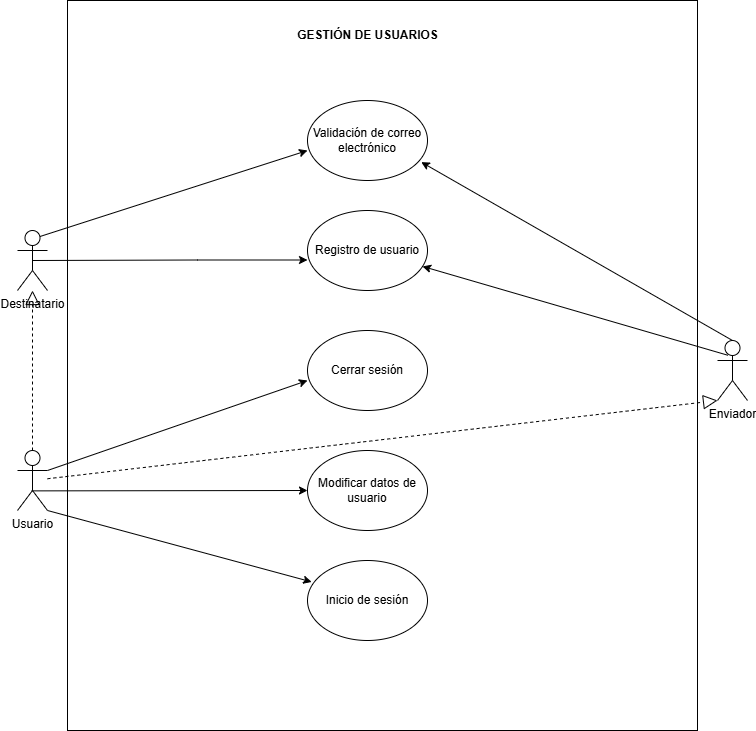
\includegraphics[width=0.9\textwidth]{imagenes/Analisis/Gestion de usuarios.png}
    \caption{Diagrama de casos de uso: Gestión de usuarios}
    \label{fig:gestion_usuarios}
\end{figure}

\newpage
\subsection{Gestión de remesas}
\begin{figure}[H]
    \centering
    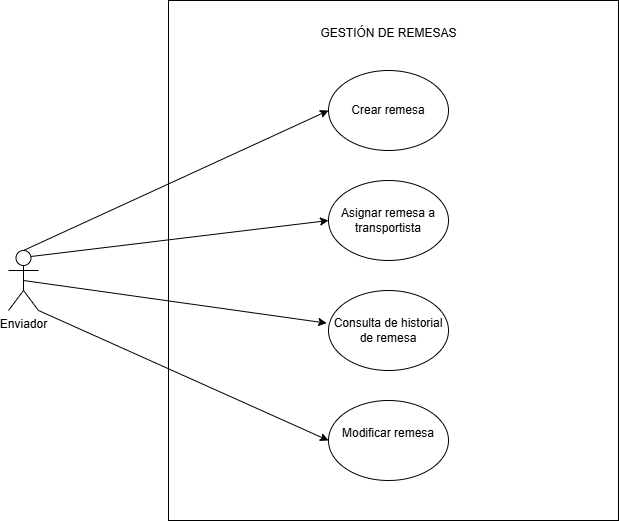
\includegraphics[width=0.9\textwidth]{imagenes/Analisis/gestionderemesas.png}
    \caption{Diagrama de casos de uso: Gestión de remesas}
    \label{fig:gestion_remesas}
\end{figure}

\subsection{Gestión de seguimiento y localización}
\begin{figure}[H]
    \centering
    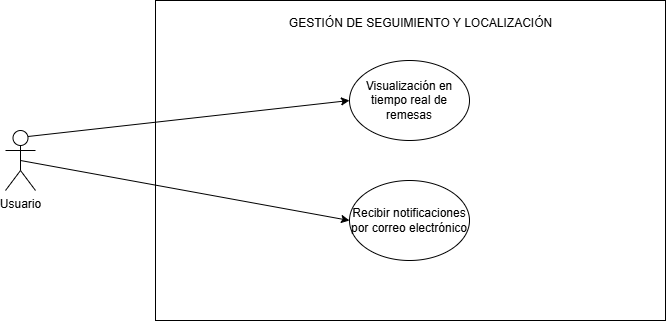
\includegraphics[width=0.9\textwidth]{imagenes/Analisis/gestiondeseguimientoylocalizacion.png}
    \caption{Diagrama de casos de uso: Gestión de seguimiento y localización}
    \label{fig:gestion_seguimiento_localizacion}
\end{figure}

\newpage
\subsection{Gestión de transportistas}
\begin{figure}[H]
    \centering
    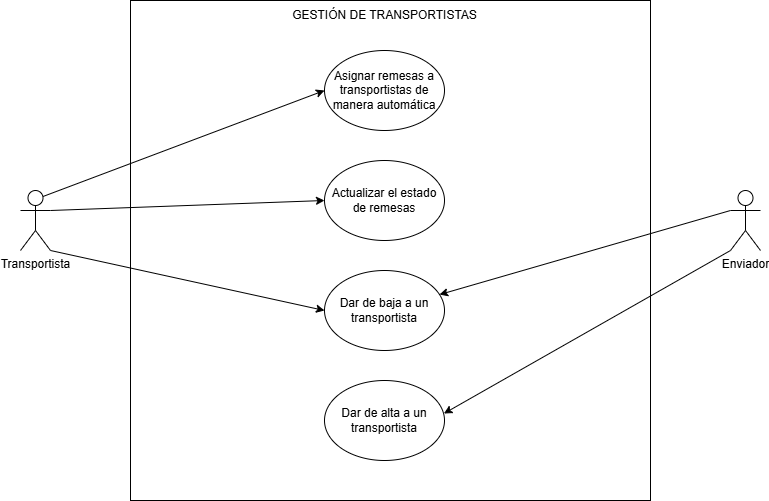
\includegraphics[width=0.9\textwidth]{imagenes/Analisis/gestiondetransportistas.png}
    \caption{Diagrama de casos de uso: Gestión de transportistas}
    \label{fig:gestion_transportistas}
\end{figure}

\subsection{Gestión de estadísticas y reportes}
\begin{figure}[H]
    \centering
    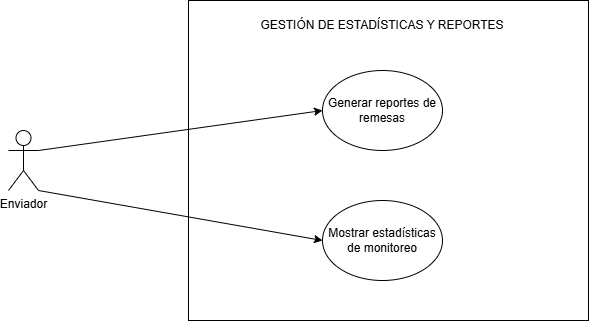
\includegraphics[width=0.9\textwidth]{imagenes/Analisis/gestionDeEstadisticasyReportes.png}
    \caption{Diagrama de casos de uso: Gestión de estadísticas y reportes}
    \label{fig:gestion_estisticas_reportes}
\end{figure}

\newpage
\subsection{Gestión de la blockchain}
\begin{figure}[H]
    \centering
    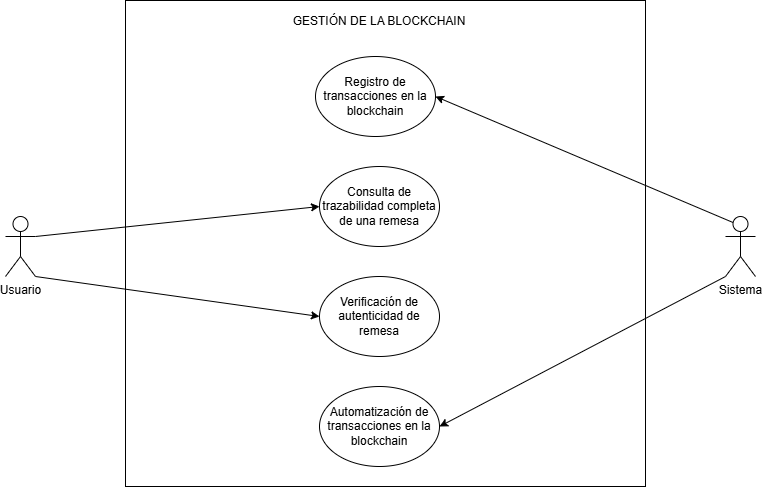
\includegraphics[width=0.9\textwidth]{imagenes/Analisis/gestionDeLaBlockchain.png}
    \caption{Diagrama de casos de uso: Gestión de la blockchain}
    \label{fig:gestion_blockchain}
\end{figure}

